\documentclass[9pt,twocolumn]{paper-template}
% Use the lineno option to display guide line numbers if required.

\usepackage{lipsum}
\usepackage{hyperref}
\newcommand{\cirbd}{\mathrel{\text{\faDotCircle[regular]}}}
\newcommand{\ofatdot}{\mathbin{\tikz{\draw[line width=0.25pt] (0,0) circle[radius=0.7ex];\draw[fill] (0,0) circle[radius=0.3ex];}}}




\templatetype{twocolumn} % Choose template 
% {pnasresearcharticle} = Template for a two-column research article
% {pnasmathematics} %= Template for a one-column mathematics article
% {pnasinvited} %= Template for a PNAS invited submission

\title{Farsi handwritten digit recognition}

% Use letters for affiliations, numbers to show equal authorship (if applicable) and to indicate the corresponding author

\author[a]{Mohammad Mohammad Beigi}


\affil[a]{Student, Department, Sharif University of Technology}


% Please add here a significance statement to explain the relevance of your work


% Please include corresponding author, author contribution and author declaration information


% Keywords are not mandatory, but authors are strongly encouraged to provide them. If provided, please include two to five keywords, separated by the pipe symbol, e.g:
\keywords{Keywords: Hoda Dataset  $|$ sumfilter $|$ maxfilter $|$ SVM $|$ d'} 

\begin{abstract}

In this research article, we have a brief overview on addressing a significant gap in existing literature by delving into the realm of Farsi handwritten digit recognition. Our investigation involves a comprehensive study of various classification and feature extraction techniques, offering a detailed performance analysis. 

 A meticulous evaluation comprising 54 distinct classifier/feature combinations is conducted, focusing on accuracy and classification time for Arabic digits. The findings are scrutinized, revealing a specific challenge associated with the digit '0,' for which we propose an effective resolution method. 
 


\end{abstract}

\dates{This manuscript was compiled on \today}

\begin{document}

\maketitle
\thispagestyle{firststyle}
\ifthenelse{\boolean{shortarticle}}{\ifthenelse{\boolean{singlecolumn}}{\abscontentformatted}{\abscontent}}{}

% If your first paragraph (i.e. with the \dropcap) contains a list environment (quote, quotation, theorem, definition, enumerate, itemize...), the line after the list may have some extra indentation. If this is the case, add \parshape=0 to the end of the list environment.
\dropcap{I}



n the realm of pattern recognition and machine learning, the handwritten digit recognition problem stands as a noteworthy subtask within the broader landscape of Optical Character Recognition (OCR). While OCR encompasses a wide range of applications, there exists a distinct category that demands precision and rapidity in recognizing digits, such as postal codes and bank checks reading. In these specialized applications, the emphasis is on achieving exceptionally high accuracy and speed in the identification of numerical characters.

Furthermore, the handwritten digit recognition problem assumes a pivotal role beyond its specific applications. It serves as a valuable benchmark for evaluating and comparing various classification techniques. The challenge of deciphering handwritten digits not only addresses practical use cases but also provides a standardized testing ground for assessing the efficacy of different algorithms and methodologies in the domain of pattern recognition. This article explores the nuances of the handwritten digit recognition problem, delving into its applications, challenges, and its pivotal role as a benchmark for advancing classification techniques.


In the expansive landscape of handwritten character recognition, substantial research has been dedicated to deciphering Latin digits, with a myriad of techniques extensively explored and documented [1–8]. However, a noticeable gap emerges when it comes to Arabic handwritten digit recognition, where research endeavors have been comparatively limited. Notably, Al-Omari et al. [9] contributed to this nascent field by proposing a system tailored for the recognition of Arabic digits spanning from '1' to '9'. Their approach involved the utilization of a feature vector endowed with scale-, translation-, and rotation-invariant properties. Training a probabilistic neural network (PNN) on this distinctive feature set, their work marked a significant stride in addressing the specific challenges posed by Arabic handwritten digits.

As the research community grapples with the complexities of handwritten digit recognition, the dearth of studies in the realm of Arabic digits underscores an unexplored frontier. The work of Al-Omari et al. not only addresses this gap but also introduces a methodology that extends beyond the conventional focus on Latin characters. This adds a layer of diversity to the recognition landscape, prompting a closer examination of the challenges and opportunities unique to Arabic handwritten digit recognition. This article delves into the existing body of research, shedding light on the distinctive features and methodologies employed in the recognition of Arabic handwritten digits, with an aim to foster a deeper understanding of this underexplored domain.





\section*{Materials and Methods}


\subsection*{Dataset}

Hoda dataset is the first dataset of handwritten Farsi digits that has been developed during an MSc. project in Tarbiat Modarres University entitled: Recognizing Farsi Digits and Characters in SANJESH Registration Forms. This project has been carried out in cooperation with Hoda System Corporation. It was finished in summer 2005 under supervision of Prof. Ehsanollah Kabir. Samples of the dataset are handwritten characters extracted from about 12000 registration forms of university entrance examination in Iran. The dataset specifications is as follows:\\
\begin{itemize}
	\item Resolution of samples: 200 dpi
	\item Total samples: 102,352 samples
	\item Training samples: 60,000 samples
	\item Test samples: 20,000 samples
\item 	Remaining samples: 22,352 samples
\end{itemize}

Samples with different writing styles in the dataset are shown in Fig 1.

\begin{figure}[h!]
	\centering
	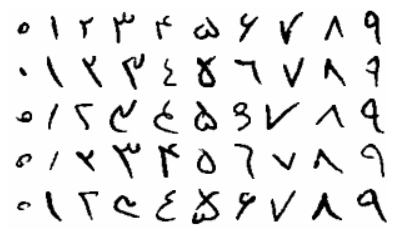
\includegraphics[width=\linewidth]{figures/screenshot001}
	\caption{Samples with different writing styles}
	\label{fig:frog}
\end{figure}

\newpage

\section*{Classification Methods}


\section*{Nearest Mean}



The Nearest Mean Classifier is a simple and intuitive algorithm used for classification tasks. It's also known as the Nearest Centroid Classifier or the Nearest Prototype Classifier. The basic idea behind this classifier is to assign a new data point to the class whose mean (centroid) is nearest to the point in the feature space.

Here's a step-by-step explanation of how the Nearest Mean Classifier works:

1. Training Phase:\\
For each class in the training dataset, calculate the mean (centroid) of the feature vectors belonging to that class. The mean is computed by averaging the values of each feature across all instances in that class.

\[ \mu_i = \frac{1}{\text{N}} \sum_{i=1}^{\text{N}} F_i \]

Where $\mu_i$ is Mean of class i, N is Number of instances in class, and F is Feature vector.


2. Testing Phase:\\
Given a new data point (feature vector), calculate the distance between the feature vector and the mean of each class. The distance can be measured using various metrics, such as Euclidean distance or Manhattan distance.

\[ \text{D}_{\text{class}} = \text{D}(\text{F}, \mu_{\text{class}}) \]

where D is Distance from class

3. Classification:
- Assign the new data point to the class whose mean is the closest in terms of distance.

\[ \text{Predicted Class} = \arg\min_{\text{class}} \left(\text{D}_{\text{class}}\right) \]

The Nearest Mean Classifier assumes that the classes are roughly spherical and have similar covariance matrices. This makes the algorithm computationally efficient and easy to implement. However, it may not perform well if the underlying assumptions are not met, for example, in cases where classes have different variances or shapes.

It's worth noting that the Nearest Mean Classifier is sensitive to outliers because the mean can be heavily influenced by extreme values. In practice, data preprocessing and normalization can be applied to mitigate this sensitivity.






\section*{K-Nearest Neighbors (KNN)}

K-Nearest Neighbors (KNN) is a simple and intuitive supervised machine learning algorithm used for classification and regression tasks. In the context of classification, I'll explain how the KNN classifier works:

\subsection*{Basic Concept:}
\begin{enumerate}
	\item \textbf{Instance Space:} Imagine your data points plotted in a multi-dimensional space, where each point represents an instance characterized by its features.
	
	\item \textbf{Classification by Proximity:} KNN classifies a new data point based on the majority class of its K nearest neighbors. "K" is a user-defined parameter.
\end{enumerate}

\subsection*{Workflow:}
\begin{enumerate}
	\item \textbf{Training:}
	\begin{itemize}
		\item Store all training examples.
		\item No explicit training phase occurs in KNN; it memorizes the entire training dataset.
	\end{itemize}
	
	\item \textbf{Prediction:}
	\begin{itemize}
		\item Given a new data point, find its K nearest neighbors in the training set.
		\item Typically, Euclidean distance is used for measuring proximity, but other distance metrics can be used as well.
		\item Assign the class label to the new data point based on the majority class among its K nearest neighbors.
	\end{itemize}
\end{enumerate}

\subsection*{Key Parameters:}
\begin{itemize}
	\item \textbf{K (Number of Neighbors):} It is crucial to choose an appropriate value for K. A small K may be sensitive to noise, while a large K might smooth out decision boundaries.
\end{itemize}

\subsection*{Considerations:}
\begin{itemize}
	\item \textbf{Distance Metric:} The choice of distance metric can impact the performance of KNN. Common choices include Euclidean distance, Manhattan distance, or other similarity measures.
	
	\item \textbf{Feature Scaling:} KNN is sensitive to the scale of features. It's often a good practice to normalize or standardize features to ensure equal importance.
\end{itemize}

\subsection*{Pros and Cons:}
\subsubsection*{Pros:}
\begin{itemize}
	\item Simple to implement and understand.
	\item No training phase, as it memorizes the entire training dataset.
	\item Non-parametric, meaning it makes no assumptions about the underlying data distribution.
\end{itemize}

\subsubsection*{Cons:}
\begin{itemize}
	\item Computationally expensive, especially for large datasets.
	\item Sensitive to irrelevant or redundant features.
	\item The optimal choice of K and the distance metric may vary for different datasets.
\end{itemize}

\subsection*{Example:}
Suppose you have a dataset with two features (e.g., height and weight) and two classes (e.g., "Male" and "Female"). If you have a new data point (height, weight), KNN would classify it based on the majority class among its K nearest neighbors in the training data.

In summary, KNN is a versatile algorithm suitable for small to moderately sized datasets, and its performance can be influenced by the choice of parameters and the nature of the data.



\section*{Gaussian Naive Bayes classifier}





\textbf{Naive Bayes Classifier:}
Naive Bayes is a family of probabilistic algorithms based on the Bayes theorem, which describes the probability of an event based on prior knowledge of conditions that might be related to the event. It is considered ``naive'' because it makes the assumption that the features used to describe an observation are independent, given the class label.

\textbf{Gaussian Naive Bayes Classifier:}
The Gaussian Naive Bayes classifier is a specific instance of the Naive Bayes classifier where it is assumed that the features follow a Gaussian (normal) distribution. This means that the likelihood of the features given the class is modeled as a Gaussian distribution.

In the context of classification, here's a simplified explanation of how the Gaussian Naive Bayes classifier works:

\begin{enumerate}
	\item \textbf{Data and Features:}
	Given a dataset with labeled examples, each example has multiple features (variables) associated with it.
	
	\item \textbf{Training:}
	The classifier estimates the mean and standard deviation of each feature for each class.
	
	\item \textbf{Gaussian Distribution:}
	It assumes that the values of features for each class are normally (Gaussian) distributed.
	
	\item \textbf{Probability Calculation:}
	To classify a new observation, the algorithm calculates the probability of the observation belonging to each class using the Gaussian probability density function.
	
	\item \textbf{Decision Rule:}
	The class with the highest probability is assigned as the predicted class for the new observation.
\end{enumerate}

The key assumption of independence between features can be quite strong, and in practice, it might not hold for many real-world datasets. Despite this limitation, Gaussian Naive Bayes is known to perform well in various classification tasks, especially when the independence assumption is not severely violated.

Keep in mind that if your question was referring to a specific variant or implementation of a Gaussian Bayes classifier that differs from the typical Gaussian Naive Bayes, please provide more details for a more accurate response.



\section*{The Parzen Window Classifier}

The Parzen Window classifier is a non-parametric technique used for pattern recognition and classification. It falls under the category of kernel density estimation methods. The main idea behind the Parzen Window classifier is to estimate the probability density function (PDF) of the underlying data by placing a window (or kernel) at each data point and summing up the contributions from all data points within the window.

\subsection*{Step-by-Step Explanation}

\begin{enumerate}[label={\arabic*.}, font=\bfseries]
	
	\item \textbf{Data Representation:}
	\begin{itemize}
		\item Let's say you have a dataset with labeled samples, where each sample belongs to a particular class.
	\end{itemize}
	
	\item \textbf{Kernel Function:}
	\begin{itemize}
		\item Choose a kernel function, typically a symmetric probability density function, such as the Gaussian (normal) distribution. The choice of the kernel function influences the shape of the window and the smoothness of the estimated density.
	\end{itemize}
	
	\item \textbf{Window Placement:}
	\begin{itemize}
		\item For each data point in the dataset, place a window centered at that point. The window's size (bandwidth) determines how much influence nearby points have on the classification.
	\end{itemize}
	
	\item \textbf{Density Estimation:}
	\begin{itemize}
		\item Calculate the contribution of each data point to the probability density estimation within its corresponding window using the chosen kernel function. The contributions are summed up for all data points.
	\end{itemize}
	
	\item \textbf{Classification:}
	\begin{itemize}
		\item To classify a new data point, place a window centered at that point and calculate the density estimation based on nearby training samples. The class with the highest estimated density is assigned to the new data point.
	\end{itemize}
	
	\item \textbf{Parameter Tuning:}
	\begin{itemize}
		\item The performance of the Parzen Window classifier is influenced by the choice of the kernel function and the window size. The bandwidth of the window determines how much smoothing is applied to the density estimation. Cross-validation or other model selection techniques can be used to choose optimal parameters.
	\end{itemize}
	
\end{enumerate}

One of the advantages of the Parzen Window classifier is its simplicity and flexibility. However, it may not perform well in high-dimensional spaces due to the curse of dimensionality, as the volume of the space increases exponentially with dimensionality. Additionally, the performance can be sensitive to the choice of kernel and bandwidth.




\section*{Feature Extraction Methods}





\section*{Horizontal Histogram }

A horizontal histogram of an image is a graphical representation that shows the distribution of pixel intensities along the horizontal axis of the image. In other words, it provides a visual summary of how many pixels in each intensity level exist across the width of the image.

\subsection*{Step-by-step Explanation}

\begin{enumerate}
	\item \textbf{Pixel Intensities:} Each pixel in a grayscale image has a certain intensity value, typically ranging from 0 (black) to 255 (white). In a color image, the intensity values are often represented in separate channels (e.g., red, green, blue).
	
	\item \textbf{Horizontal Axis:} The horizontal axis of the histogram represents the range of pixel intensities. The leftmost part usually corresponds to the lowest intensity (e.g., 0), and the rightmost part corresponds to the highest intensity (e.g., 255).
	
	\item \textbf{Vertical Axis:} The vertical axis of the histogram represents the frequency or the number of pixels at each intensity level. Higher peaks indicate more pixels with that intensity.
	
	\item \textbf{Creation:} To create a horizontal histogram, you consider each row of pixels in the image independently. For each intensity level, you count how many pixels in that row have that intensity. The result is a set of values that form a horizontal line or curve.
	
	\item \textbf{Visualization:} These values are then plotted along the horizontal axis, creating a graph that visually represents the distribution of pixel intensities across the image's width. Peaks in the histogram indicate prevalent intensity levels, and valleys represent less common intensities.
\end{enumerate}

\textbf{Analysis and Applications:}\\
Analyzing the horizontal histogram can provide insights into the overall brightness distribution across the width of the image. For example, a well-balanced histogram might indicate a well-exposed image, while an uneven histogram might suggest overexposed or underexposed areas. Image processing techniques often use histograms for tasks like contrast enhancement, equalization, and thresholding.

\section*{Vertical Histogram }



A vertical histogram of an image is a graphical representation that illustrates the distribution of pixel intensities along the vertical axis of the image. It is similar to a horizontal histogram but focuses on the pixel intensities along the image's height rather than its width.

\subsection*{Key Points}

\begin{enumerate}
	\item \textbf{Pixel Intensities:} Similar to a horizontal histogram, each pixel in a grayscale image has a certain intensity value, usually ranging from 0 (black) to 255 (white). In color images, intensity values are often represented in separate channels, such as red, green, and blue.
	
	\item \textbf{Vertical Axis:} The vertical axis of the histogram represents the range of pixel intensities. The bottom part typically corresponds to the lowest intensity (e.g., 0), and the top part corresponds to the highest intensity (e.g., 255).
	
	\item \textbf{Horizontal Axis:} The horizontal axis of the histogram represents the frequency or the number of pixels at each intensity level along the image's height. Peaks indicate prevalent intensity levels in the image, while valleys represent less common intensities.
	
	\item \textbf{Creation:} To create a vertical histogram, you consider each column of pixels in the image independently. For each intensity level, you count how many pixels in that column have that intensity. The result is a set of values that form a vertical line or curve.
	
	\item \textbf{Visualization:} These values are then plotted along the vertical axis, creating a graph that visually represents the distribution of pixel intensities across the image's height. Peaks in the histogram indicate prevalent intensity levels along the image's height, and valleys represent less common intensities.
\end{enumerate}

\textbf{Analysis and Applications}\\
Analyzing the vertical histogram can provide insights into the overall brightness distribution along the height of the image. It can be useful in identifying patterns, uneven illumination, or other characteristics that may impact image quality. Similar to horizontal histograms, vertical histograms are employed in image processing tasks for functions like contrast enhancement, equalization, and thresholding.

\section*{Wavelet}


Wavelet features are a type of feature extraction technique that is used to extract essential information from a signal or image. Wavelet transform is applied to the image, either directly or on the gradient decomposition of the image. This helps in reducing the dimensionality of the problem and can lead to faster classification. Wavelet transform can also help in reducing noise and non-essential information, improving the classification performance. In the context of Arabic handwritten digit recognition, the image is resized and composed into three resolution levels, and the third level approximation of the image is used as wavelet features, resulting in a feature vector of 64 elements.

\section*{Zoning}

In the employed methodology, the image undergoes a uniform partitioning into zones measuring 5×5, as elucidated in reference. Subsequently, the average value of each individual zone is computed, resulting in the generation of a feature vector comprising 25 elements. 

\section*{Results}

After learning Procedure we obtain 4 matrices named "XTrain", "XTest", "ytrain" and "ytest" which contains examples and labels of train and test sets.

\section{First part}



In this part We train the data set on Head and Medium body and test on Far and Close body.(Actually at first I divided the images wrongly and ran the model. I thought that it is better if I don't put the created data away )


\subsection*{Nearest Neighbor Classifier}

We use a  Nearest Neighbor Classifier to calculate the accuracy of the predictions of the model. (figure 1)



As you see similar to SVM, accuracy is significantly higher than NN Classifier but mostly less than using SVM
classifier.(figure 7)

Note that number of trees does not affect the result significantly.








\newpage
	

\section*{Second part}
	
	
	
	In this part We train the data set on Head and also test on Head.(So here we train on 75 targets and 75 distractors and also test on 75 targets and 75 distractors)
	
		


\subsection*{Nearest Neighbor Classifier}



As you see we obtained accuracy 0.5067 by NNC.(figure 8)

\subsection*{Support Vector Machine Classifier}



Parameters of SVM model are as in figure 9.


As you see accuracy is higher than NN Classifier.(figure 10)

\subsection*{Random Forest Classifier}


As you see similar to SVM, accuracy is significantly higher than NN Classifier and more than using SVM
classifier.(figure 11)




\section*{Third part}



In this part We train the data set on Close body and also test on Close body.(So here we train on 75 targets and 75 distractors and also test on 75 targets and 75 distractors)




\subsection*{Nearest Neighbor Classifier}





As you see we obtained accuracy 0.4645 by NNC.(figure 12)

\subsection*{Support Vector Machine Classifier}
Parameters of SVM model are as in figure 13.





As you see accuracy is significantly less than NN Classifier.(figure 14)

\subsection*{Random Forest Classifier}



As you see similar to SVM, accuracy is significantly less than NN Classifier and more than using SVM
classifier.(figure 15)








\section*{Forth part}





In this part We train the data set on Far body and also test on Far body.(So here we train on 75 targets and 75 distractors and also test on 75 targets and 75 distractors)




\subsection*{Nearest Neighbor Classifier}






As you see we obtained accuracy 0.4645 by NNC.(figure 16)

\subsection*{Support Vector Machine Classifier}
Parameters of SVM model are as in figure 17.



As you see accuracy is significantly higher than NN Classifier.(figure 18)

\subsection*{Random Forest Classifier}



As you see similar to SVM, accuracy is significantly higher than NN Classifier but less than using SVM
classifier.(figure 19)






\section*{5th part}





In this part We train the data set on Medium body and also test on Medium body.(So here we train on 75 targets and 75 distractors and also test on 75 targets and 75 distractors)




\subsection*{Nearest Neighbor Classifier}




As you see we obtained accuracy 0.5828 by NNC.(figure 20)

\subsection*{Support Vector Machine Classifier}
Parameters of SVM model are as in figure 21.



As you see accuracy is higher than NN Classifier.(figure 22)

\subsection*{Random Forest Classifier}



As you see similar to SVM, accuracy is significantly less than both NN Classifier and  SVM
classifier.(figure 23)



\section*{6th part}


Here we train the model on 300 targets and 300 distractors and test it on other 300 targets and 300 distractors. 


\subsection*{Nearest Neighbor Classifier}




As you see we obtained accuracy 0.5350 by NNC.(figure 24)

\subsection*{Support Vector Machine Classifier}

Parameters of SVM model are as in figure 25.



As you see accuracy is higher than NN Classifier.(figure 26)


\subsection*{Random Forest Classifier}



As you see similar to SVM, accuracy is significantly less than both NN Classifier and  SVM
classifier.(figure 27)



\subsection*{ROC}

Figure 28 is ROC curve of the  model  tested on 600 test images.

Now we plot ROC for first 75 test target images which are close body(figure 29).




Now we plot ROC for second 75 test target images which are far body(figure 30).



Now we plot ROC for second 75 test target images which are Head(figure 31).





Now we plot ROC for second 75 test target images which are Medium body(figure 32).







\subsection*{d primes}


d' for these five datasets are as in figure 33.



We have plotted d' in figure 34. As you see it changes across datasets as same as the figure in article.



			
			
			
			
			
\section{Conclusion}	

In the figures created in this homework we observed that mostly SVM classifier is the strongest classifier after learning procedure by Hmax model. We also calculated ROC for different views of body and showed that d' is higher for close body(as same as the article).

 We also ran the model separately for each view and observed different classifiers performance while just one view have been in the learning procedure.
 
 One phenomena of this homework was the first part of results that we obtained an accuracy which was approximately 20\% higher than running the model on regular structure of dataset. In this part we trained the data set on Head and Medium body and tested on Far and Close body.
			
			
			Further more also could run the model and investigate its accuracy on noisy images. We use salt and pepper noise or gaussian noise.
			

\showacknow{} % Display the acknowledgments section

\section*{References}
% Bibliography
%\bibliography{references}

1. A feedforward architecture accounts
for rapid categorization; Thomas Serre, Aude Oliva, and Tomaso Poggio
			
	2.Hubel DH, Wiesel TN (1968) J Phys 195:215–243.
	
	
3.	Perrett D, Oram M (1993) Image Vision Comput 11:317–333.

	4. Kobatake E, Tanaka K (1994) J Neurophysiol 71:856–867.
	
	5. Tanaka K (1996) Annu Rev Neurosci 19:109–139.	
	

\end{document}